\chapter{Производная и линейное приближение}\label{chap:c20}\markright{Глава 40}
\section{От средней скорости к мгновенной}

\par\addvspace{5pt}\begin{lrbox}{\CatFlowBox}\begin{minipage}[t]{\linewidth}
\setlength{\parskip}{5pt}\setlength{\columnsep}{4.5mm}\setlength{\intextsep}{0pt}
\begin{wrapfigure}[9]{r}{54mm}

\includegraphics[width=54mm,height=58mm,keepaspectratio]{images/unique/art-55.png}
\label{catflow:55}
\end{wrapfigure}
Если известны два показания координаты движущегося тела, можно найти среднюю скорость изменения координаты: разделить её изменение на прошедшее время. При длинном промежутке времени такая средняя скрывает подробности движения. Для описания отдельного момента рассматривают всё более короткие промежутки около него и выясняют, к какому числу приближаются средние скорости. Это та же идея предела, теперь применённая к специально составленному отношению. Она пригодна не только для движения: так можно описывать изменение площади при изменении стороны и изменение затрат при небольшом увеличении объёма производства.

Геометрически два значения функции задают две точки графика. Проходящая через них прямая показывает средний наклон между этими точками. Когда вторая точка приближается к первой, такой наклон иногда имеет конечный предел. Тогда появляется прямая, передающая поведение графика вблизи одной точки. При этом приближается именно отношение изменений: малость числителя и знаменателя по отдельности ещё не определяет результат деления.
\par\WFclear\end{minipage}\end{lrbox}%
\ifdim\dimexpr\ht\CatFlowBox+\dp\CatFlowBox\relax<64mm\dp\CatFlowBox=\dimexpr64mm-\ht\CatFlowBox\relax\fi%
\noindent\usebox{\CatFlowBox}\par\addvspace{5pt}
\begin{definition}
\term{Приращение аргумента} (increment of the argument) в точке \(a\) --- число \(h\), задающее новый аргумент \(a+h\). Соответствующее \term{приращение функции} (increment of the function) равно \(f(a+h)-f(a)\).
\end{definition}

\begin{definition}
\term{Секущая} (secant line) через различные точки графика с аргументами \(a\) и \(a+h\), где \(h\ne0\), имеет угловой коэффициент
\[
\frac{f(a+h)-f(a)}h.
\]
\end{definition}

\begin{definition}
\term{Производная в точке} (derivative at a point) \(a\) --- конечный предел
\[
f'(a)=\lim_{h\to0}\frac{f(a+h)-f(a)}h,
\]
если он существует. Здесь функция определена в некотором открытом промежутке около \(a\). Тогда функцию называют \term{дифференцируемой} (differentiable) в \(a\). Проверка только одного знака приращения даёт одностороннюю производную, а не полную проверку этого определения.
\end{definition}

\begin{definition}
Если \(f'(a)\) существует, \term{касательная} (tangent line) к графику в точке \((a;f(a))\) задаётся формулой
\[
y=f(a)+f'(a)(x-a).
\]
\end{definition}

\begin{example}
При \(f(x)=x^2\) разностное отношение равно
\[
\frac{(a+h)^2-a^2}{h}=2a+h\quad(h\ne0).
\]
Следовательно, \(f'(a)=2a\). В точке \(a=1\) касательная имеет уравнение \(y=1+2(x-1)=2x-1\). Приращение \(h\) бывает и отрицательным: предел с обеих сторон один и тот же.
\end{example}

\section{Когда производная существует}

\begin{theorem}[Дифференцируемость и непрерывность]\label{thm:legacy-c20-1}
Если функция дифференцируема в \(a\), то она непрерывна в \(a\).
\end{theorem}
\begin{proof}
При \(h\ne0\) имеем
\[
f(a+h)-f(a)=h\,\frac{f(a+h)-f(a)}h.
\]
Первый множитель стремится к нулю, второй --- к конечному \(f'(a)\). По правилу произведения приращение функции стремится к нулю, что и означает непрерывность.
\end{proof}

Обратное утверждение неверно. Для \(f(x)=|x|\) в нуле разностное отношение равно \(\frac{|h|}{h}\): справа оно равно \(1\), слева \(-1\). Функция непрерывна, но производной в нуле нет. Для корня в начале его области определения правое отношение \(\frac{\sqrt h}{h}=\frac1{\sqrt h}\) при \(h>0\) неограниченно растёт. Оно также не даёт конечной производной.

\section{Первые формулы из определения}

\begin{theorem}[Простейшие производные]\label{thm:legacy-c20-2}
Производная постоянной функции равна нулю, а производная \(f(x)=x\) равна единице. Для натурального \(n\ge2\)
\[
(x^n)'=nx^{n-1}.
\]
При \(x>0\) выполнено \((\sqrt x)'=\frac1{2\sqrt x}\).
\end{theorem}
\begin{proof}
У постоянной числитель разностного отношения нулевой. Для \(f(x)=x\) отношение равно \(1\). Для степени применим доказанный в главе \ref{chap:c19} предел \(\frac{x^n-a^n}{x-a}\) при \(x\to a\): замена \(x=a+h\) даёт определение производной в \(a\). Для корня при \(a>0\) домножение на сопряжённое даёт
\[
\frac{\sqrt{a+h}-\sqrt a}{h}=\frac1{\sqrt{a+h}+\sqrt a}\to\frac1{2\sqrt a}.
\]
Оба последних вычисления опираются на арифметику пределов, а не на готовую таблицу.
\end{proof}

Например, \((x^3)'=3x^2\), \((x^5)'=5x^4\). В обозначении \(f'(x)\) аргумент \(x\) пробегает точки, в которых производная существует; так получается новая функция. Запись \(f'(a)\) обозначает её значение в выбранной точке.

\section{Алгебра производных}

\begin{theorem}[Сумма, произведение и частное]\label{thm:legacy-c20-3}
Пусть \(f\) и \(g\) дифференцируемы в \(a\), а \(\alpha,\beta\) --- действительные постоянные. Тогда
\[
(\alpha f+\beta g)'(a)=\alpha f'(a)+\beta g'(a),
\]
\[
(fg)'(a)=f'(a)g(a)+f(a)g'(a).
\]
Если \(g(a)\ne0\), то в некоторой окрестности частное определено и
\[
\left(\frac fg\right)'(a)=\frac{f'(a)g(a)-f(a)g'(a)}{g(a)^2}.
\]
\end{theorem}
\par\addvspace{5pt}\begin{lrbox}{\CatFlowBox}\begin{minipage}[t]{\linewidth}
\setlength{\parskip}{5pt}\setlength{\columnsep}{4.5mm}\setlength{\intextsep}{0pt}
\begin{wrapfigure}[12]{l}{54mm}

\includegraphics[width=54mm,height=58mm,keepaspectratio]{images/unique/art-56.png}
\label{catflow:56}
\end{wrapfigure}
\textit{Доказательство.} Для линейной комбинации разностное отношение распадается на линейную комбинацию двух разностных отношений; используем правило суммы пределов. Для произведения прибавим и вычтем \(f(a)g(a+h)\). После деления на \(h\ne0\) получаем
\[
\frac{f(a+h)-f(a)}h\,g(a+h)
+f(a)\,\frac{g(a+h)-g(a)}h.
\]
Непрерывность \(g\), следующая из её дифференцируемости, разрешает предельный переход и даёт формулу произведения. Если \(g(a)\ne0\), её непрерывность обеспечивает ненулевой знаменатель возле \(a\). Для функции \(\frac1g\) отношение приращений равно
\[
-\frac{g(a+h)-g(a)}{h\,g(a+h)g(a)}
\to-\frac{g'(a)}{g(a)^2}.
\]
Применив правило произведения к \(f\) и \(\frac1g\), получаем правило частного.\hfill\(\blacksquare\)
\par\WFclear\end{minipage}\end{lrbox}%
\ifdim\dimexpr\ht\CatFlowBox+\dp\CatFlowBox\relax<64mm\dp\CatFlowBox=\dimexpr64mm-\ht\CatFlowBox\relax\fi%
\noindent\usebox{\CatFlowBox}\par\addvspace{5pt}


Умножение функций отличается от умножения их производных. Например, производная \(x\cdot x\) равна \(2x\), хотя произведение двух производных равно \(1\). Для частного важно проверять знаменатель до преобразований: в исключённой точке исходная функция не становится определённой оттого, что её запись удалось сократить.

\begin{example}
Для \(f(x)=\frac{x+1}{x-2}\), \(x\ne2\),
\[
f'(x)=\frac{(x-2)-(x+1)}{(x-2)^2}=-\frac3{(x-2)^2}.
\]
Здесь обе исходные производные равны единице, но производная частного вовсе не равна их частному.
\end{example}

\section{Сложная функция}

\par\addvspace{5pt}\begin{lrbox}{\CatFlowBox}\begin{minipage}[t]{\linewidth}
\setlength{\parskip}{5pt}\setlength{\columnsep}{4.5mm}\setlength{\intextsep}{0pt}
\begin{wrapfigure}[11]{r}{54mm}

\includegraphics[width=54mm,height=58mm,keepaspectratio]{images/unique/art-96.png}
\label{catflow:96}
\end{wrapfigure}
Правило цепочки позволяет вычислять производную композиции, не раскрывая её в длинное выражение. Внешнюю и внутреннюю функции нужно определить до вычислений. Например, в \((3x^2-1)^4\) внешняя функция возводит число в четвёртую степень, а внутренняя даёт \(3x^2-1\). Производная внутреннего выражения остаётся отдельным множителем. Правило работает и тогда, когда внутреннее приращение равно нулю для некоторых малых шагов: это специально учтено в следующем доказательстве.
\par\WFclear\end{minipage}\end{lrbox}%
\ifdim\dimexpr\ht\CatFlowBox+\dp\CatFlowBox\relax<64mm\dp\CatFlowBox=\dimexpr64mm-\ht\CatFlowBox\relax\fi%
\noindent\usebox{\CatFlowBox}\par\addvspace{5pt}
\begin{theorem}[Правило цепочки; chain rule]\label{thm:legacy-c20-4}
Пусть \(g\) дифференцируема в \(a\), \(b=g(a)\), а \(f\) дифференцируема в \(b\). Предполагается, что композиция определена в окрестности \(a\). Тогда
\[
(f\circ g)'(a)=f'(g(a))g'(a).
\]
\end{theorem}
\begin{proof}
Обозначим \(A=g'(a)\), \(B=f'(b)\). Определение производной позволяет записать
\[
g(a+h)-b=h\bigl(A+\alpha(h)\bigr),\qquad \alpha(h)\to0,
\]
\[
f(b+k)-f(b)=k\bigl(B+\beta(k)\bigr),\qquad \beta(k)\to0.
\]
При ненулевых приращениях функции \(\alpha\) и \(\beta\) равны ошибкам соответствующих разностных отношений. Положим \(\beta(0)=0\), тогда второе равенство верно и при \(k=0\), а \(\beta\) непрерывна в нуле. Подставим \(k=g(a+h)-b\). Непрерывность \(g\) даёт \(k\to0\), а непрерывность \(\beta\) --- \(\beta(k)\to0\). Отношение приращения композиции к \(h\) равно \((A+\alpha(h))(B+\beta(k))\) и стремится к \(AB\). Это рассуждение включает случай, когда внутреннее приращение иногда равно нулю; делить на него не требуется.
\end{proof}

Например,
\[
\bigl((3x^2-1)^4\bigr)'=4(3x^2-1)^3\cdot6x
=24x(3x^2-1)^3.
\]
Сначала дифференцируется внешняя четвёртая степень, затем результат умножается на производную внутреннего выражения. Для \(\sqrt{2x+3}\) получаем \(\frac1{\sqrt{2x+3}}\) при \(x>-\frac32\); на границе этого промежутка приведённое вычисление не применяется.

Следующая короткая таблица содержит только уже обоснованные случаи. В строках с \(n\) число \(n\) натуральное.
\[
\begin{array}{c|c|c}
\text{Функция}&\text{Производная}&\text{Условие}\\ \hline
c&0&x\in\mathbb R\\
x&1&x\in\mathbb R\\
x^n&nx^{n-1}&n\ge2,\ x\in\mathbb R\\
\frac1{x^n}&-\frac n{x^{n+1}}&x\ne0\\
\sqrt x&\frac1{2\sqrt x}&x>0
\end{array}
\]
Для отрицательных целых степеней строка получается из правила частного. Производная любого многочлена теперь вычисляется по слагаемым, рациональной функции --- по правилу частного, а композиции этих выражений --- по правилу цепочки с проверкой области определения.

\section{Линейное приближение и его ошибка}

Касательная полезна не только как линия на рисунке. Её формула заменяет сложную зависимость простой линейной зависимостью вблизи выбранной точки. Сначала нужно выбрать точку, где значение функции и производную легко вычислить. Затем находят небольшое приращение аргумента и умножают его на производную. Полученная поправка прибавляется к известному значению функции. Чем именно оправдано такое вычисление, показывает определение производной: после вычитания линейной поправки остаётся ошибка, которая при уменьшении приращения становится малой даже по сравнению с самим приращением.

Это локальное утверждение: оно относится к достаточно близким аргументам около фиксированной точки. Само определение не выдаёт готового численного допуска для любого выбранного шага. Для гарантированной оценки ошибки нужно дополнительно оценить остаток у конкретной функции. Полезно также сохранять единицы измерения: производная показывает изменение результата на единицу изменения аргумента, поэтому произведение производной на приращение имеет те же единицы, что и значение функции.

\begin{definition}
\term{Линейное приближение} (linear approximation) дифференцируемой функции возле \(a\) --- выражение \(f(a)+f'(a)h\) для оценки \(f(a+h)\), где \(h\) мало по модулю. Запись \(f(a+h)\approx f(a)+f'(a)h\) обозначает приближение, а не точное равенство.
\end{definition}

\begin{theorem}[Точный смысл линейного приближения]\label{thm:legacy-c20-5}
Если \(f\) дифференцируема в \(a\), то
\[
f(a+h)=f(a)+f'(a)h+r(h),\qquad
\lim_{h\to0}\frac{r(h)}h=0.
\]
\end{theorem}
\begin{proof}
Положим \(r(h)=f(a+h)-f(a)-f'(a)h\). При \(h\ne0\) частное \(\frac{r(h)}h\) равно разностному отношению функции минус его предел \(f'(a)\), поэтому стремится к нулю. Это также означает \(\frac{|r(h)|}{|h|}\to0\).
\end{proof}

У корня удобно взять \(a=4\): значение равно \(2\), производная --- \(\frac14\). Поэтому
\[
\sqrt{4+h}\approx2+\frac h4,\qquad
\sqrt{4{,}04}\approx2{,}01.
\]
Для квадрата точный остаток особенно прост: \((a+h)^2=a^2+2ah+h^2\). Ошибка линейного приближения равна \(h^2\), а её отношение к \(|h|\) равно \(|h|\) и стремится к нулю.

\section{Скорость, затраты и проверка экстремума}

Если \(s(t)\) --- координата в метрах, а \(t\) измеряется в секундах, то \(s'(t)\) --- \term{мгновенная скорость изменения координаты} (instantaneous velocity) в метрах в секунду. Знак показывает направление движения вдоль выбранной оси; модуль даёт величину скорости. Если \(C(q)\) --- затраты в рублях при непрерывно изменяемом объёме \(q\), то \(C'(q)\) описывает малое изменение затрат на единицу изменения объёма. Для целого числа изделий такое использование производной даёт оценку модели, которую можно сравнить с точной разностью \(C(q+1)-C(q)\).

\begin{definition}
Точка \(a\) является точкой \term{локального минимума} (local minimum), если в некоторой её окрестности все допустимые значения \(f(x)\) не меньше \(f(a)\). Для \term{локального максимума} (local maximum) они не больше \(f(a)\). Оба случая называют \term{локальным экстремумом} (local extremum).
\end{definition}

\begin{theorem}[Ферма; Fermat's theorem]\label{thm:legacy-c20-6}
Если \(a\) --- внутренняя точка области определения, функция дифференцируема в \(a\) и имеет в ней локальный экстремум, то \(f'(a)=0\).
\end{theorem}
\par\addvspace{5pt}\begin{lrbox}{\CatFlowBox}\begin{minipage}[t]{\linewidth}
\setlength{\parskip}{5pt}\setlength{\columnsep}{4.5mm}\setlength{\intextsep}{0pt}
\begin{wrapfigure}[13]{l}{54mm}

\includegraphics[width=54mm,height=58mm,keepaspectratio]{images/unique/art-70.png}
\label{catflow:70}
\end{wrapfigure}
\textit{Доказательство.} В случае минимума при малых \(h>0\) отношение \(\frac{f(a+h)-f(a)}h\) неотрицательно, а при малых \(h<0\) неположительно. По предельному переходу в неравенствах общий предел одновременно неотрицателен и неположителен, значит, равен нулю. Для максимума знаки меняются местами, а вывод остаётся тем же.\hfill\(\blacksquare\)
\par\WFclear\end{minipage}\end{lrbox}%
\ifdim\dimexpr\ht\CatFlowBox+\dp\CatFlowBox\relax<64mm\dp\CatFlowBox=\dimexpr64mm-\ht\CatFlowBox\relax\fi%
\noindent\usebox{\CatFlowBox}\par\addvspace{5pt}


\term{Стационарная точка} (stationary point) --- внутренняя точка, в которой производная существует и равна нулю. К \term{критическим точкам} (critical points) здесь относят стационарные точки и внутренние точки области определения, в которых производной нет. Теорема Ферма задаёт необходимое условие для дифференцируемого экстремума, но не достаточное: у \(x^3\) в нуле производная нулевая, а значения слева отрицательны, справа положительны, поэтому экстремума нет.

Сначала монотонность конкретной функции проверяем сравнением значений, а экстремум --- прямой оценкой. Например, если \(0\le x<y\), то \(y^2-x^2=(y-x)(y+x)>0\); значит, квадрат строго возрастает на \([0;+\infty)\). При \(x<y\le0\) та же разность отрицательна, поэтому квадрат строго убывает на \((-\infty;0]\). Для функции \(P(q)=300-(q-20)^2\) сразу получаем \(P(q)\le300\) с равенством только при \(q=20\). Так проверяется максимум, предложенный уравнением \(P'(q)=0\).

При поиске наибольшего значения на заданном отрезке нужно учитывать и концы: у \(f(x)=x\) на \([0;1]\) наибольшее значение равно \(1\), хотя производная нигде не нулевая. В точке \(0\) функция \(|x|\) имеет минимум без производной. Поэтому вывод о конкретном экстремуме должен сопровождаться проверкой значений или оценкой, действительной в нужной области.

\section{Применение правил к новым функциям}
Пользуясь табличными производными синуса, косинуса и экспоненты вместе с доказанным правилом частного, получаем
\[
(\operatorname{ctg}x)'=-\frac1{\sin^2x}\quad(\sin x\ne0),
\]
\[
(\operatorname{th}x)'=\frac1{\operatorname{ch}^2x},\qquad
(\operatorname{cth}x)'=-\frac1{\operatorname{sh}^2x}\quad(x\ne0).
\]
Например, числитель производной \(\frac{\operatorname{sh}x}{\operatorname{ch}x}\) равен \(\operatorname{ch}^2x-\operatorname{sh}^2x=1\). Для гиперболического котангенса порядок меняется, и числитель равен \(-1\). Полная таблица находится в начале книги; правила получения новых производных изучаются здесь.

\section{Теоремы о среднем значении}
\begin{theorem}[Ролль; Rolle's theorem]\label{thm:legacy-c29-5}
Если \(g\) непрерывна на \([a;b]\), дифференцируема на \((a;b)\) и \(g(a)=g(b)\), то существует \(c\in(a;b)\) с \(g'(c)=0\).
\end{theorem}
\begin{proof}
Если функция постоянна, подойдёт любая внутренняя точка. Иначе хотя бы одно из наибольшего и наименьшего значений, существующих по теореме Вейерштрасса, отличается от общего значения на концах. Оно достигается внутри. По теореме Ферма из главы \ref{chap:c20} производная там равна нулю.
\end{proof}
\begin{theorem}[Лагранж; mean value theorem]\label{thm:legacy-c29-6}
Если \(g\) непрерывна на \([a;b]\) и дифференцируема на \((a;b)\), то для некоторого \(c\in(a;b)\)
\[
g(b)-g(a)=g'(c)(b-a).
\]
В частности, функция с нулевой производной на интервале постоянна на нём.
\end{theorem}
\begin{proof}
Применим теорему Ролля к \(h(x)=g(x)-g(a)-\frac{g(b)-g(a)}{b-a}(x-a)\). Она равна нулю на концах, а равенство \(h'(c)=0\) даёт нужную формулу. Если \(g'=0\), применяем формулу к любым двум точкам интервала.
\end{proof}
\section{Исследование функции с помощью производной}
\begin{theorem}[Знак производной и монотонность]
Пусть функция непрерывна на промежутке и дифференцируема в его внутренних точках. Если всюду внутри \(f'>0\), функция строго возрастает; если \(f'<0\), строго убывает. При \(f'\ge0\) функция не убывает, при \(f'\le0\) не возрастает.
\end{theorem}
\begin{proof}Для любых двух точек \(x_1<x_2\) применяем теорему Лагранжа на \([x_1;x_2]\): \(f(x_2)-f(x_1)=f'(c)(x_2-x_1)\). Положительность второго множителя переносит соответствующий знак производной на разность значений.\end{proof}
\begin{theorem}[Достаточное условие экстремума]
Пусть \(f\) непрерывна в \(a\) и дифференцируема по обе стороны в некоторой проколотой окрестности. Если знак производной при переходе через \(a\) меняется с плюса на минус, в \(a\) строгий локальный максимум. При смене с минуса на плюс --- строгий локальный минимум.
\end{theorem}
\begin{proof}В первом случае функция строго возрастает слева к значению \(f(a)\) и строго убывает справа от него; непрерывность позволяет включить граничную точку в сравнение. Во втором случае знаки обратные.\end{proof}
\par\addvspace{2pt}\begin{lrbox}{\CatFlowBox}\begin{minipage}[t]{\linewidth}
\setlength{\parskip}{2pt}\setlength{\columnsep}{4.5mm}\setlength{\intextsep}{0pt}
\begin{wrapfigure}[11]{l}{54mm}

\includegraphics[width=54mm,height=58mm,keepaspectratio]{images/unique/art-254.png}
\label{catflow:254}
\end{wrapfigure}
Исследование через производную начинается с области определения функции, а затем --- области существования производной. Нули производной и точки её отсутствия разбивают область на промежутки, на которых можно определить знак. В таблице знаков необходимо различать нуль функции, нуль производной и запрещённую точку: это три разных события. Для поиска наибольшего и наименьшего значений на отрезке сравнивают значения во внутренних критических точках и на обоих концах. Если критических точек конечное число, это конечный список кандидатов; его полнота следует из теоремы Ферма и существования экстремумов у непрерывной функции на отрезке. На открытом или неограниченном промежутке отдельно исследуют граничные пределы и достижимость предполагаемой грани.
\par\WFclear\end{minipage}\end{lrbox}%
\ifdim\dimexpr\ht\CatFlowBox+\dp\CatFlowBox\relax<58mm\dp\CatFlowBox=\dimexpr58mm-\ht\CatFlowBox\relax\fi%
\noindent\usebox{\CatFlowBox}\par\addvspace{2pt}
\begin{example}Пусть \(f(x)=x^3-3x\). Производная \(3(x-1)(x+1)\) положительна вне \([-1;1]\) и отрицательна внутри. Поэтому \(x=-1\) --- точка максимума со значением \(2\), а \(x=1\) --- точка минимума со значением \(-2\). На отрезке \([-2;3]\) сравниваем \(f(-2)=-2,f(-1)=2,f(1)=-2,f(3)=18\). Наибольшее значение \(18\), наименьшее \(-2\), причём минимум достигается при двух разных аргументах.\end{example}
\begin{example}Для \(f(x)=\ln x-x\) область \(x>0\), производная \(\frac1x-1=\frac{1-x}x\). Она положительна до единицы и отрицательна после. Глобальный максимум \(-1\) достигается при \(x=1\). Наибольшее значение обосновано монотонностью на всей области, а не одним равенством \(f'(1)=0\).\end{example}
\section{Графики функции и её производной}
\begin{definition}\term{Ускорение} (\emph{acceleration}) одномерного движения с дважды дифференцируемой координатой \(s(t)\) равно \(a(t)=s''(t)\). Знак координатной скорости \(s'\) задаёт направление; величина скорости равна \(|s'|\).\end{definition}
\begin{example}На графике производной выше горизонтальной оси функция возрастает, ниже --- убывает. Площадь под графиком самой производной связана с изменением функции в главе \ref{chap:c29}. По высоте графика \(f'\) нельзя сразу найти высоту \(f\): прибавление постоянной к функции не меняет производную. Для касательной с угловым коэффициентом \(k\) ищем \(f'(a)=k\), затем подставляем точку \((a;f(a))\) в \(y=f(a)+k(x-a)\).\end{example}
\begin{center}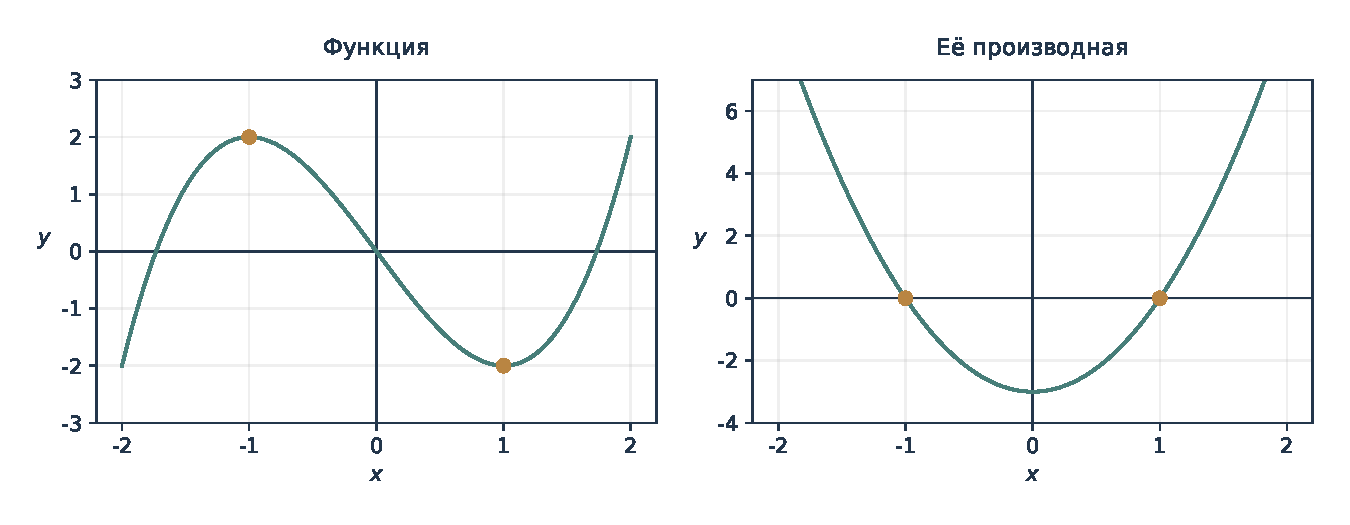
\includegraphics[width=\linewidth,height=74mm,keepaspectratio]{images/exam-calculus-signs.pdf}\end{center}
\par\addvspace{2pt}\begin{lrbox}{\CatFlowBox}\begin{minipage}[t]{\linewidth}
\setlength{\parskip}{2pt}\setlength{\columnsep}{4.5mm}\setlength{\intextsep}{0pt}
\begin{wrapfigure}[9]{r}{54mm}

\includegraphics[width=54mm,height=58mm,keepaspectratio]{images/unique/art-255.png}
\label{catflow:255}
\end{wrapfigure}
В задаче по рисунку сначала установи, что именно изображено: сама функция, её производная или касательная. Нули производной находятся в общих точках её графика с горизонтальной осью, но сами по себе не гарантируют экстремума исходной функции. Смена знака производной с плюса на минус является достаточным признаком строгого локального максимума, а с минуса на плюс --- строгого локального минимума при условиях доказанной теоремы. Если производная лишь касается оси и остаётся положительной, функция продолжает возрастать. Концы указанного отрезка участвуют в поиске абсолютного максимума независимо от того, равна ли там производная нулю. Знак второй производной показывает изменение координатной скорости, но увеличение модуля скорости требует совместного учёта знаков первой и второй производных. Эти различия позволяют объяснить ответ по графику, а не угадывать его по внешнему сходству кривых.
\par\WFclear\end{minipage}\end{lrbox}%
\ifdim\dimexpr\ht\CatFlowBox+\dp\CatFlowBox\relax<58mm\dp\CatFlowBox=\dimexpr58mm-\ht\CatFlowBox\relax\fi%
\noindent\usebox{\CatFlowBox}\par\addvspace{2pt}
\relax

\par\addvspace{2pt}\begin{lrbox}{\CatFlowBox}\begin{minipage}[t]{\linewidth}
\setlength{\parskip}{2pt}\setlength{\columnsep}{4.5mm}\setlength{\intextsep}{0pt}
\begin{wrapfigure}[13]{l}{54mm}

\includegraphics[width=54mm,height=58mm,keepaspectratio]{images/unique/art-269.png}
\label{catflow:269}
\end{wrapfigure}
График производной задаёт скорость изменения функции, но не её абсолютную высоту. При добавлении к функции постоянной производная остаётся прежней. При применении достаточного признака экстремума проверяют смену знака производной по сторонам точки; для нахождения самого значения функции нужны дополнительные данные. Касание графика производной оси не обязательно меняет знак и не обязательно даёт экстремум исходной функции. Наклон касательной вычисляют по двум её точкам, даже если они не лежат на графике функции. Когда в условии выделен отрезок, сначала отмечают его концы: экстремумы за его пределами не участвуют в подсчёте, а сравнение значений на концах требует отдельного шага.
\par\WFclear\end{minipage}\end{lrbox}%
\ifdim\dimexpr\ht\CatFlowBox+\dp\CatFlowBox\relax<61mm\dp\CatFlowBox=\dimexpr61mm-\ht\CatFlowBox\relax\fi%
\noindent\usebox{\CatFlowBox}\par\addvspace{2pt}
\relax
\section{Рисунок производной и рисунок касательной}
На графике \(f^{\prime}\) высота показывает скорость изменения \(f\), а не само значение \(f\). При подсчёте экстремумов учитывают направление смены знака и принадлежность аргумента указанному промежутку. Касание графика \(f^{\prime}\) горизонтальной оси без смены знака может дать стационарную точку без экстремума. У касательной угловой коэффициент находят по двум точкам прямой: \(\frac{y_2-y_1}{x_2-x_1}\). Отношение \(y/x\) подходит только для прямой через начало координат.
\begin{center}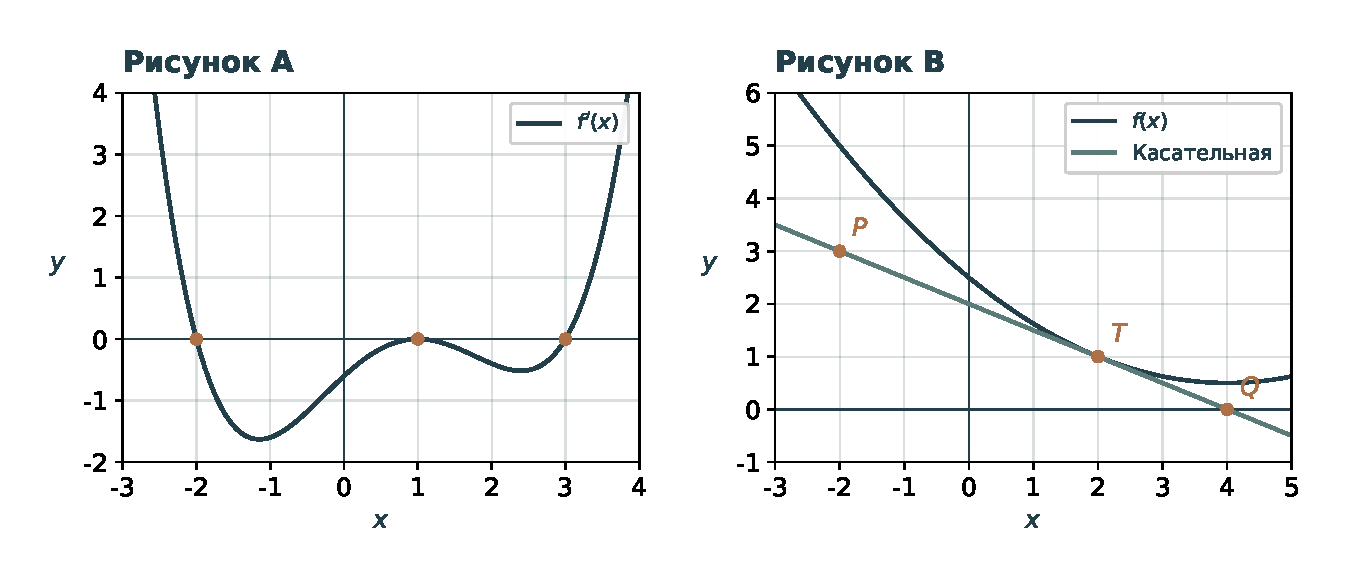
\includegraphics[width=\linewidth,height=78mm,keepaspectratio]{images/review-ege-calculus.pdf}\end{center}

\section{Составной экстремум: преобразовать до дифференцирования}
\begin{example}[Тригонометрические слагаемые могут сократиться в производной]\label{ex:review-ege-c20-1}
Для \(f(x)=(x-1)\cos x-\sin x\) на \([0;\pi]\) правило произведения даёт
\[
f^{\prime}(x)=\cos x-(x-1)\sin x-\cos x=(1-x)\sin x.
\]
Во внутренности отрезка \(\sin x>0\). Поэтому функция возрастает до \(1\) и убывает после \(1\); максимум \(f(1)=-\sin1\). Для минимума сравним концы: \(f(0)=-1\), \(f(\pi)=1-\pi<-1\), поскольку \(\pi>2\). Минимум \(1-\pi\) при \(x=\pi\). Нуль производной на конце сам по себе не определяет характер абсолютного экстремума.
\end{example}
\begin{example}[Мощность и достижимая оценка]\label{ex:review-ege-c20-2}
При нагрузке \(R>0\) пусть \(P(R)=\frac{100R}{(R+2)^2}\). Из \((R+2)^2\ge8R\) следует \(P\le\frac{25}{2}\). Равенство при \(R=2\) допустимо, значит, максимум \(\frac{25}{2}\). Проверка производной даёт \(P^{\prime}(R)=\frac{100(2-R)}{(R+2)^3}\), то же возрастание и убывание. Выбор положительной области является частью модели.
\end{example}
\begin{example}[Замена обратного квадрата в модели амплитуды]\label{ex:review-ege-c20-3}
Для \(t>0\) задана положительная величина
\[
A(t)=\frac{2t^2}{\sqrt{(9-t^2)^2+9t^2}}.
\]
Знаменатель положителен при всех \(t>0\). Возводя в квадрат и деля на \(t^4\), получаем
\[
A(t)^2=\frac4{81u^2-9u+1},\qquad u=\frac1{t^2}>0.
\]
Знаменатель \(81(u-\frac1{18})^2+\frac34\) минимален при допустимом \(u=\frac1{18}\). Поэтому \(t=3\sqrt2\), а \(A_{\max}=\frac4{\sqrt3}\). Нельзя просто минимизировать исходный знаменатель: числитель тоже зависит от \(t\). Замена сохраняет всю область, поскольку каждому \(u>0\) соответствует ровно одно \(t>0\).
\end{example}
\par\noindent\begin{minipage}{\linewidth}\section*{Графики}
\begin{center}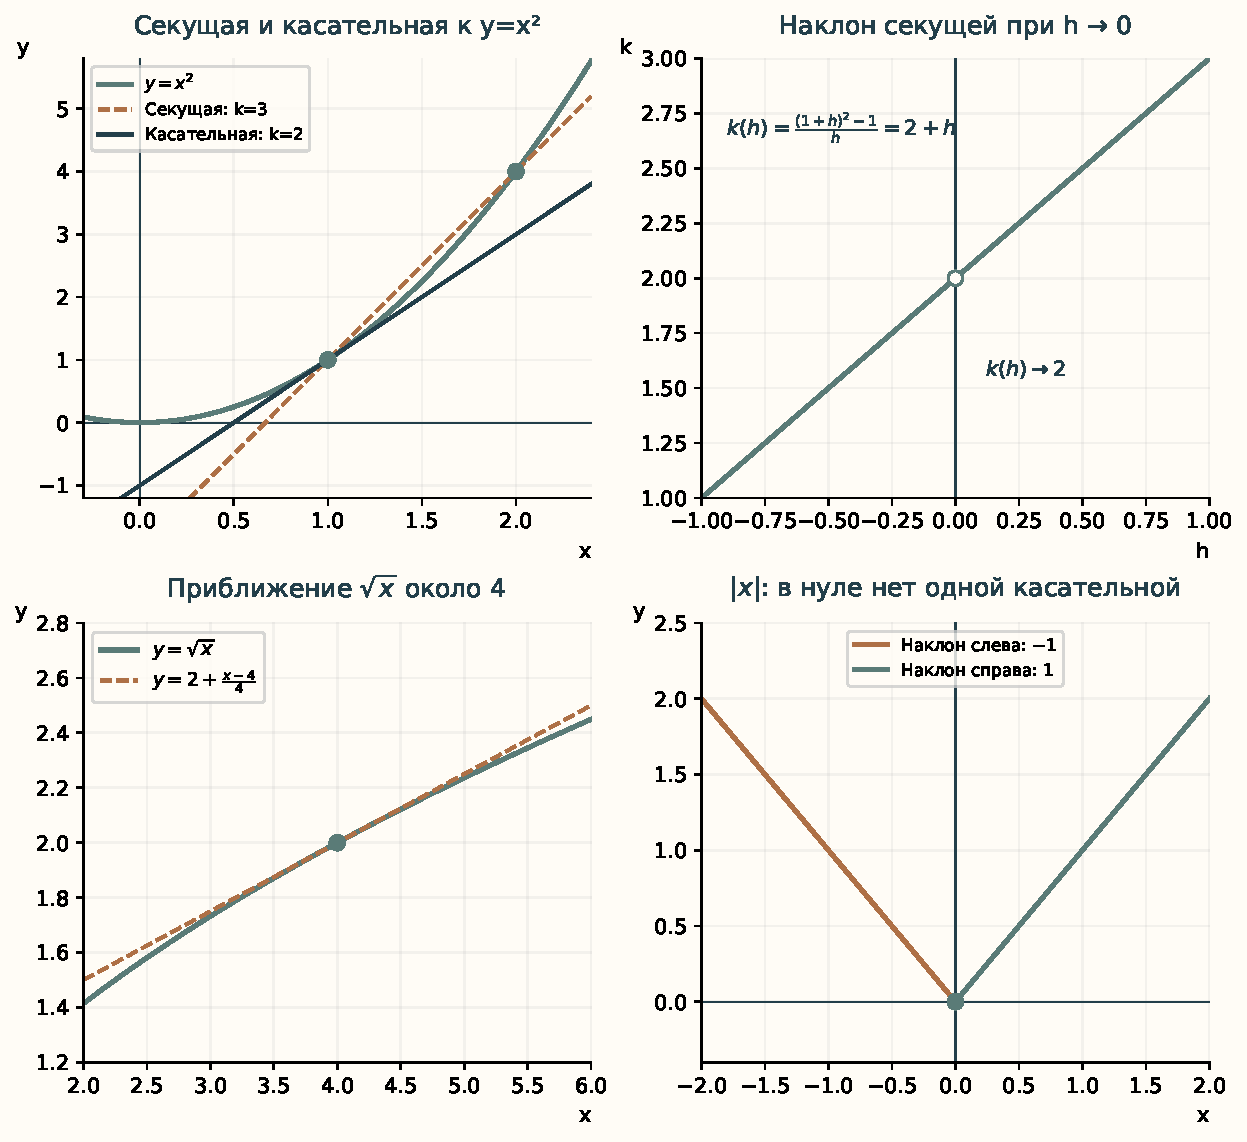
\includegraphics[width=\textwidth,height=.79\textheight,keepaspectratio]{images/atlas-derivative.pdf}\par\small Наклон и линейное приближение\end{center}\end{minipage}\par
\Needspace{7\baselineskip}\section*{Задачи}
\begingroup\setlength{\parskip}{2pt}
\noindent\begin{minipage}[t]{\linewidth}\textbf{40.1.} Для \(f(x)=x^2\) вычисли \(f'(3)\) непосредственно по определению производной.\par\end{minipage}\par
\noindent\begin{minipage}[t]{\linewidth}\textbf{40.2.} Для \(f(x)=x^3\) вычисли \(f'(-2)\), раскрыв куб в разностном отношении.\par\end{minipage}\par
\noindent\begin{minipage}[t]{\linewidth}\textbf{40.3.} Найди производную \(5x^4-3x^2+7\).\par\end{minipage}\par
\noindent\begin{minipage}[t]{\linewidth}\textbf{40.4.} Найди производную \((2x+1)(x^2-3)\) по правилу произведения и проверь раскрытием скобок.\par\end{minipage}\par
\noindent\begin{minipage}[t]{\linewidth}\textbf{40.5.} Найди производную \(f(x)=\dfrac{x+1}{x-2}\) и укажи её область определения.\par\end{minipage}\par
\noindent\begin{minipage}[t]{\linewidth}\textbf{40.6.} Найди производную \(\sqrt x\) в точке \(9\) по определению, используя сопряжённое выражение.\par\end{minipage}\par
\noindent\begin{minipage}[t]{\linewidth}\textbf{40.7.} Найди производную \((3x^2-1)^4\). Укажи внешнюю и внутреннюю функции.\par\end{minipage}\par
\noindent\begin{minipage}[t]{\linewidth}\textbf{40.8.} Найди производную \(\sqrt{2x+3}\) во внутренних точках области определения.\par\end{minipage}\par
\noindent\begin{minipage}[t]{\linewidth}\textbf{40.9.} Запиши уравнение касательной к графику \(y=x^3\) в точке с аргументом \(1\).\par\end{minipage}\par
\noindent\begin{minipage}[t]{\linewidth}\textbf{40.10.} Проверь существование производной \(f(x)=|x|\) в точке \(0\), вычислив разностное отношение с двух сторон.\par\end{minipage}\par
\noindent\begin{minipage}[t]{\linewidth}\textbf{40.11.} Найди стационарные точки \(f(x)=x^3-3x\). Проверь наличие локальных экстремумов прямой факторизацией \(f(x)-f(a)\) в каждой найденной точке.\par\end{minipage}\par
\par\addvspace{5pt}\begin{lrbox}{\CatFlowBox}\begin{minipage}[t]{\linewidth}
\setlength{\parskip}{5pt}\setlength{\columnsep}{4.5mm}\setlength{\intextsep}{0pt}
\begin{wrapfigure}[9]{r}{54mm}

\includegraphics[width=54mm,height=58mm,keepaspectratio]{images/unique/art-57.png}
\label{catflow:57}
\end{wrapfigure}
\textbf{40.12.} Докажи прямым сравнением значений, что \(x^3\) строго возрастает на всей прямой. Объясни, почему \(f'(0)=0\) этому не мешает.\par

\textbf{40.13.} Координата тела задана \(s(t)=t^3-6t^2+12t\) метров при \(t\ge0\) секунд. Найди мгновенную скорость изменения координаты при \(t=1\) и \(t=2\).\par

\textbf{40.14.} В непрерывной модели затраты равны \(C(q)=100+5q+0{,}02q^2\) рублей. При \(q=50\) оцени приращение затрат на одно дополнительное изделие через производную и сравни с точной разностью.\par

\textbf{40.15.} Сторону квадратной площадки увеличивают с \(10\) до \(10{,}02\) метра. Оцени прирост площади линейным приближением и найди его точное значение.\par

\textbf{40.16.} Длина натянутого троса в модели равна \(L(x)=\sqrt{x^2+9}\) метров. При \(x=4\) метра оцени изменение длины, если горизонтальный отступ увеличится на \(0{,}1\) метра.\par

\textbf{40.17.} Модель прибыли \(P(q)=-q^2+40q-100\) задана при \(0\le q\le30\). Найди точку, предлагаемую уравнением \(P'(q)=0\), и докажи, что в ней прибыль наибольшая, выделив полный квадрат.\par

\textbf{40.18.} Оцени \(\sqrt{16{,}08}\) линейным приближением функции \(\sqrt x\) возле \(16\).\par
\par\WFclear\end{minipage}\end{lrbox}%
\ifdim\dimexpr\ht\CatFlowBox+\dp\CatFlowBox\relax<64mm\dp\CatFlowBox=\dimexpr64mm-\ht\CatFlowBox\relax\fi%
\noindent\usebox{\CatFlowBox}\par\addvspace{5pt}

\noindent\begin{minipage}[t]{\linewidth}\textbf{40.19.} Докажи непосредственно по определению, что производная постоянной функции \(f(x)=c\) равна нулю.\par\end{minipage}\par
\noindent\begin{minipage}[t]{\linewidth}\textbf{40.20.} Докажи: если в точке \(a\) существует конечная производная, то \(f(a+h)-f(a)\to0\) при \(h\to0\).\par\end{minipage}\par
\noindent\begin{minipage}[t]{\linewidth}\textbf{40.21.} Пусть функция чётная на открытом промежутке около \(0\) и дифференцируема в \(0\). Докажи, что \(f'(0)=0\).\par\end{minipage}\par
\noindent\begin{minipage}[t]{\linewidth}\textbf{40.22.}\starmark{} Функция равна \(x^2\) при \(x\ge0\) и \(ax+b\) при \(x<0\). Найди все \(a,b\), при которых она дифференцируема в нуле.\par\end{minipage}\par
\noindent\begin{minipage}[t]{\linewidth}\textbf{40.23.}\starmark{} Пусть \(f(x)=x|x|\). Найди производную во всех точках, включая \(0\). Является ли ноль локальным экстремумом?\par\end{minipage}\par
\noindent\begin{minipage}[t]{\linewidth}\textbf{40.24.}\starmark{} Для \(f(x)=x+\dfrac{16}{x}\), \(x>0\), найди стационарную точку. Докажи прямой оценкой, что она даёт наименьшее значение на всей области определения.\par\end{minipage}\par
\noindent\begin{minipage}[t]{\linewidth}\textbf{40.25.}\starmark{} Докажи точную формулу \(2+\dfrac h4-\sqrt{4+h}=\dfrac{h^2}{4(\sqrt{4+h}+2)^2}\) при \(h>-4\). Получи при \(0\le h\le1\) оценку ошибки между \(0\) и \(\dfrac{h^2}{64}\).\par\end{minipage}\par
\noindent\begin{minipage}[t]{\linewidth}\textbf{40.26.}\starmark{} Найди многочлен \(p(x)=ax^3+bx^2+cx+d\), касательная к которому при \(x=0\) равна \(y=1-2x\), а при \(x=1\) равна \(y=4x-1\).\par\end{minipage}\par
\noindent\begin{minipage}[t]{\linewidth}\textbf{40.27.} Найди производную \((2x^2+1)^5\).\par\end{minipage}\par
\noindent\begin{minipage}[t]{\linewidth}\textbf{40.28.} Найди производную \(\operatorname{ctg}(3x)\) и укажи область определения.\par\end{minipage}\par
\noindent\begin{minipage}[t]{\linewidth}\textbf{40.29.} Найди производную \(\operatorname{th}(x^2)\).\par\end{minipage}\par
\noindent\begin{minipage}[t]{\linewidth}\textbf{40.30.} Найди производную \(\operatorname{cth}(2x+1)\).\par\end{minipage}\par
\noindent\begin{minipage}[t]{\linewidth}\textbf{40.31.} Для \(f(x)=\dfrac{x^2+1}{x-1}\) найди \(f'(x)\) двумя способами: правилом частного и после деления многочленов.\par\end{minipage}\par
\noindent\begin{minipage}[t]{\linewidth}\textbf{40.32.}\starmark{} Докажи формулу \((f(g(h(x))))'=f'(g(h(x)))g'(h(x))h'(x)\) при дифференцируемости всех трёх функций в нужных точках.\par\end{minipage}\par
\noindent\begin{minipage}[t]{\linewidth}\textbf{40.33.} Исследуй монотонность и локальные экстремумы \(x^3-12x\).\par\end{minipage}\par
\noindent\begin{minipage}[t]{\linewidth}\textbf{40.34.} Найди наибольшее и наименьшее значения \(x^3-3x\) на \([0;2]\).\par\end{minipage}\par
\noindent\begin{minipage}[t]{\linewidth}\textbf{40.35.} Найди наибольшее значение \(xe^{-x}\) при \(x\ge0\).\par\end{minipage}\par
\noindent\begin{minipage}[t]{\linewidth}\textbf{40.36.} Исследуй \(x+\dfrac4x\) при \(x>0\) и найди минимум.\par\end{minipage}\par
\noindent\begin{minipage}[t]{\linewidth}\textbf{40.37.} Найди максимум \(\ln x-2x\), \(x>0\).\par\end{minipage}\par
\noindent\begin{minipage}[t]{\linewidth}\textbf{40.38.} Запиши касательную к \(y=\ln x\) при \(x=1\).\par\end{minipage}\par
\noindent\begin{minipage}[t]{\linewidth}\textbf{40.39.} Для \(y=x^2\) найди точку, где касательная параллельна \(y=6x+1\), и уравнение касательной.\par\end{minipage}\par
\noindent\begin{minipage}[t]{\linewidth}\textbf{40.40.} Координата \(s(t)=t^3-3t^2\), \(0\le t\le3\). Найди моменты остановки и промежутки направления движения.\par\end{minipage}\par
\noindent\begin{minipage}[t]{\linewidth}\textbf{40.41.} Для движения из предыдущей задачи найди пройденный путь за три секунды.\par\end{minipage}\par
\noindent\begin{minipage}[t]{\linewidth}\textbf{40.42.} Почему \(f'(0)=0\) у \(f(x)=x^3\) не даёт экстремума?\par\end{minipage}\par
\noindent\begin{minipage}[t]{\linewidth}\textbf{40.43.} Производная положительна на \((-2;1)\) и \((3;5)\), отрицательна на \((1;3)\); функция непрерывна на \([-2;5]\). Укажи точки локальных экстремумов внутри отрезка.\par\end{minipage}\par
\noindent\begin{minipage}[t]{\linewidth}\textbf{40.44.} На графике производной её значение в \(a\) равно \(-2\). Чему равен угловой коэффициент касательной к исходной функции? Можно ли найти \(f(a)\)?\par\end{minipage}\par
\noindent\begin{minipage}[t]{\linewidth}\textbf{40.45.}\starmark{} Докажи, что \(e^x\ge1+x\) при всех действительных \(x\).\par\end{minipage}\par
\noindent\begin{minipage}[t]{\linewidth}\textbf{40.46.}\starmark{} Докажи \(\ln x\le x-1\) при \(x>0\), укажи равенство.\par\end{minipage}\par
\noindent\begin{minipage}[t]{\linewidth}\textbf{40.47.}\starmark{} На панели A показан график производной \(f^{\prime}\); сама \(f\) дифференцируема на \((-3;4)\). Выпиши точки локального максимума и минимума \(f\), абсциссы которых принадлежат \([-\dfrac52;\dfrac72]\). Объясни роль нуля производной при \(x=1\).\par\end{minipage}\par
\noindent\begin{minipage}[t]{\linewidth}\textbf{40.48.} На панели B изображены функция и её касательная при \(x=2\). По двум отмеченным точкам касательной найди \(f^{\prime}(2)\). Можно ли вместо наклона использовать отношение ординаты точки касания к её абсциссе?\par\end{minipage}\par
\noindent\begin{minipage}[t]{\linewidth}\textbf{40.49.}\starmark{} При \(R>0\) мощность модели \(P(R)=\dfrac{144R}{(R+3)^2}\). Найди её глобальный максимум и нагрузку, при которой он достигается. Дай проверку производной.\par\end{minipage}\par
\noindent\begin{minipage}[t]{\linewidth}\textbf{40.50.}\starmark{} Найди наибольшее и наименьшее значения \(f(x)=(x-2)\cos x-\sin x\) на \([0;\pi]\).\par\end{minipage}\par
\noindent\begin{minipage}[t]{\linewidth}\textbf{40.51.}\starmark{} Для \(t>0\) задано \(A(t)=\dfrac{3t^2}{\sqrt{(16-t^2)^2+4t^2}}\). Найди глобальный максимум \(A\) и соответствующее \(t\), обосновав допустимость замены.\par\end{minipage}\par
\par\Needspace{12\baselineskip}\section*{Олимпиадные задачи}
\par\addvspace{2pt}\begin{lrbox}{\CatFlowBox}\begin{minipage}[t]{\linewidth}
\setlength{\parskip}{2pt}\setlength{\columnsep}{4.5mm}\setlength{\intextsep}{0pt}
\begin{wrapfigure}[12]{l}{54mm}

\includegraphics[width=54mm,height=58mm,keepaspectratio]{images/unique/art-319.png}
\label{catflow:319}
\end{wrapfigure}
\textbf{40.52.}\starmark{} {\small\itshape\href{https://www.imc-math.org.uk/imc1994/prob_sol.pdf}{IMC, 1994, день 1, № 2}; перевод.}\par Непрерывно дифференцируемая \(f:(a,b)\to\mathbb R\) удовлетворяет \(f(x)\to+\infty\) при \(x\to a+\), \(f(x)\to-\infty\) при \(x\to b-\) и \(f^{\prime}(x)+f(x)^2\ge-1\). Докажи \(b-a\ge\pi\) и приведи пример равенства.\par

\textbf{40.53.}\starmark{} {\small\itshape\href{https://www.imc-math.org.uk/imc1994/prob_sol.pdf}{IMC, 1994, день 2, № 1}; перевод.}\par Пусть \(f\) непрерывно дифференцируема на \([a,b]\), \(f(a)=0\), и \(|f^{\prime}(x)|\le\lambda|f(x)|\) при всех \(x\), где \(\lambda>0\). Обязательно ли \(f\equiv0\)?\par
\par\WFclear\end{minipage}\end{lrbox}%
\ifdim\dimexpr\ht\CatFlowBox+\dp\CatFlowBox\relax<58mm\dp\CatFlowBox=\dimexpr58mm-\ht\CatFlowBox\relax\fi%
\noindent\usebox{\CatFlowBox}\par\addvspace{2pt}

\endgroup
